% Figure from MATH 591 notes, section 68. Added, not from lecture (Lecture 24): the flow domain of the half-line example.
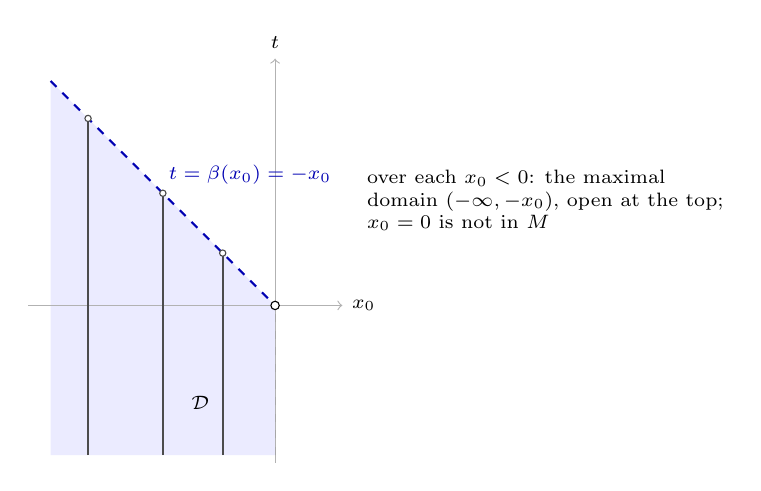
\begin{tikzpicture}[scale=0.95]
\fill[blue!8] (-3,-2) -- (-3,3) -- (0,0) -- (0,-2) -- cycle;
\draw[->, gray!60] (-3.3,0) -- (0.9,0) node[right, font=\scriptsize, text=black] {$x_0$};
\draw[->, gray!60] (0,-2.1) -- (0,3.3) node[above, font=\scriptsize, text=black] {$t$};
\draw[blue!70!black, thick, dashed] (-3,3) -- (0,0);
\draw[gray!70, dashed] (0,-2) -- (0,0);
\node[blue!70!black, font=\scriptsize, anchor=west] at (-1.55,1.75) {$t = \beta(x_0) = -x_0$};
\foreach \x in {-2.5,-1.5,-0.7} { \draw[thick, black!70] (\x,-2) -- (\x,{-\x}); \fill[white, draw=black!70] (\x,{-\x}) circle (1.2pt); }
\fill[white, draw=black] (0,0) circle (1.6pt);
\node[font=\scriptsize] at (-1.0,-1.3) {$\mathcal{D}$};
\node[font=\scriptsize, anchor=west, align=left] at (1.1,1.4) {over each $x_0 < 0$: the maximal\\ domain $(-\infty, -x_0)$, open at the top;\\ $x_0 = 0$ is not in $M$};
\end{tikzpicture}
